\documentclass[preview]{standalone}

\usepackage{amsmath}
\usepackage{amssymb}
\usepackage{bettelini}
\usepackage{stellar}
\usepackage[version=4]{mhchem}

\hypersetup{
    colorlinks=true,
    linkcolor=black,
    urlcolor=blue,
    pdftitle={Chimica},
    pdfpagemode=FullScreen,
}

\begin{document}

\title{Chimica}
\id{chimica-entalpia}
\genpage

\section{Sviluppo del calore nelle reazioni}

\plain{La rottura di un legame necessita di energia, mentre
la formazione di legami libera energia.}

\begin{snippet}{legami-energia-illustration}
    \begin{center}
    \begin{figure}[h]
        \centering
        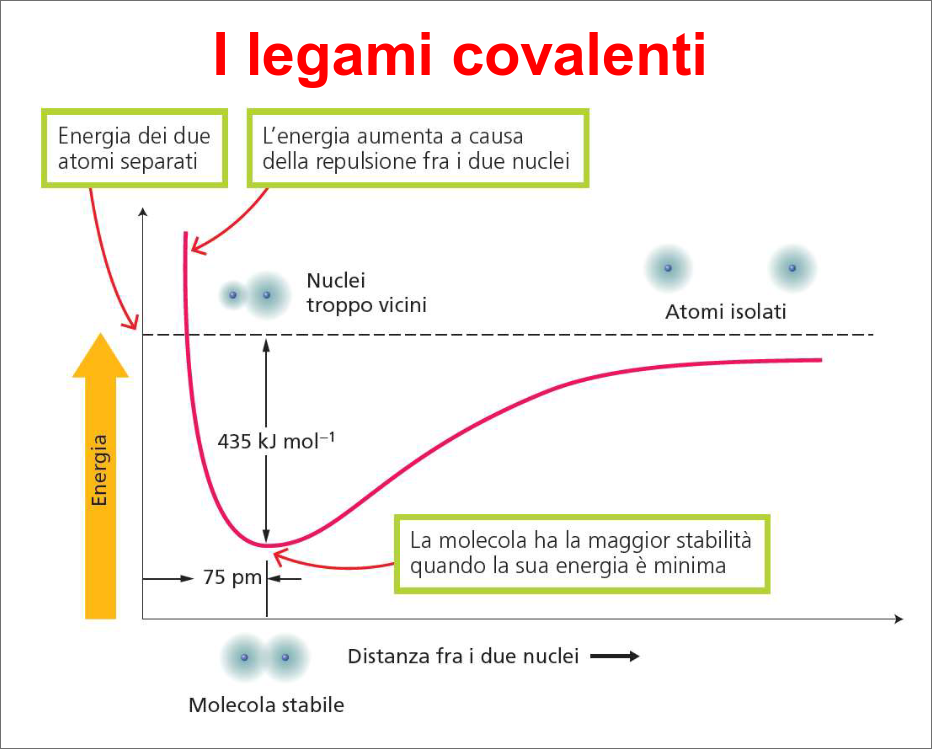
\includegraphics[width=\textwidth]{./resources/cov_bond_energy.png}
    \end{figure}
    \end{center}
\end{snippet}

\begin{snippetdefinition}{entalpia-definizione}{entalpia}
    L'\textit{entalpia} è la quantità di energia interna che un sistema
    termodinamico può scambiare con l'ambiente.
\end{snippetdefinition}

\begin{snippetdefinition}{reazione-esotermica-definizione}{Reazione esotermica}
    Una \textit{reazione esotermica} è una reazione che libera energia termica.
\end{snippetdefinition}

\begin{snippet}{reazione-esotermica-expl}
    La reazione esotermica possiede le seguenti caratteristiche:
    \begin{itemize}
        \item la reazione rilascia calore;
        \item l'ambiente circostance si scalda;
        \item l'entalpia \(\Delta H_{\text{reazione}} < 0\);
        \item i legami che si formano nei prodotti sono più forti di quelli che si rompono nei reagenti;
        \item i prodotti hanno energia inferiore rispetto ai reagenti.
    \end{itemize}
\end{snippet}

\begin{snippetdefinition}{reazione-endotermica-definizione}{Reazione endotermica}
    Una \textit{reazione endotermica} è una reazione che assorbe energia termica.
\end{snippetdefinition}

\begin{snippet}{reazione-ednotermica-expl}
    La reazione esotermica possiede le seguenti caratteristiche:
    \begin{itemize}
        \item l'entalpia \(\Delta H_{\text{reazione}} > 0\);
    \end{itemize}
\end{snippet}

\begin{snippet}{entalpia-expl1}
    In una reazione esotermica all'equilibrio chimico,
    aumentando la temperatura si sposta tale equilibrio verso i reagenti,
    per cui la reazione inversa è favorita rispetto alla reazione diretta
    per temperature elevate. Il segno della variazione di entalpia
    (che è un aspetto termodinamico) indica semplicemente la predisposizione della
    reazione chimica ad evolversi in senso diretto o inverso,
    mentre per conoscere la velocità di reazione è necessario considerare gli aspetti cinetici.
\end{snippet}

\begin{snippet}{calore-rilasciato}
    L'energia è direttamente proporzionale alle mole, e quindi alla massa.
    Il calore acquisito o rilasciato da un corpo è direttamente proporzionale
    alla variazione di temperatura a cui va incontro e si ricava dall'espressione
    \[
        Q = mc\Delta T
    \]
    dove \(c\) è il calore specifico.
\end{snippet}

\begin{snippetdefinition}{entalpia-standard-definizione}{Entalpia standard di formazione}
    L'\textit{entalpia standard di formazione}
    di una sostanza, o \textit{calore standard di formazione}
    è la quantità di calore assorbita o liberata quando una mole della sostanza
    viene formata, a \(25 {}^\circ \) C e 1 atm, dai suoi elementi nei loro stati standard.
\end{snippetdefinition}

\begin{snippet}{variazione-energia-reazione}
    Conoscendo l'entalpia delle sostanze, per qualunque
    reazione possiamo calcolare direttamente la variazione di energia di reazione.
    \[
        \Delta H^\circ_{\text{reazione}} =
        \sum_{f \in \text{prodotti}} \left( \Delta H^\circ_f \right) -
        \sum_{f \in \text{reagenti}} \left( \Delta H^\circ_f \right) 
    \]

    L'Entalpia Standard di Formazione,
    \(\Delta H^\circ_f\), di una sostanza è il \(\Delta H^\circ\)
    della sua reazione di formazione.

    Una sostanza pura ha sempre entalpia di formazione \(\Delta H^\circ_f = 0\).
\end{snippet}

\end{document}
